\chapter{INTRODUCTION}
\section{What does provenance mean in this thesis}
According to Oxford English Dictionary, provenance is the chronology of the ownership, custody or 
location of a historical object. For digital artifacts, the Provenance Working Group of World Wide 
Web Consortium (W3C) defines provenance as \begin{quote}information about entities, activities, and 
people involved in producing a piece of data or thing, which can be used to form assessments about 
its quality, reliability or trustworthiness.\end{quote} This thesis focuses on provenance for 
research publications, which are a kind of digital artifacts, so in this thesis, the word 
\emph{provenance} means information about data, their steward activities, and agents involved in the 
production of results reported in research publications. Here \emph{data} may come from observations, 
model runs or repositories supporting data reuse; \emph{data steward activities} include semantic, 
syntactical and physical changes of data; \emph{agents} are people, organizations and software agents 
relevant to the data and their steward activities at any phase of the data lifecycle; \emph{results} 
are a special kind of data that are the final products reported in papers. Note that this definition 
of results deviates from the concept of \emph{scientific conclusions}, which are hard to model.
\comment{rewrite this sentence.} Also note that information about the \emph{linkage} among these 
data, activities and agents are also implicitly included in provenance.

Semantic changes of data mean the changes in the actual content of data. Examples include data 
analysis (changing from source data to (aggregated) analysis results), data comparison (changing from 
two pieces of data to their comparison results), data verification (from data to their verification 
results) and data transformation. 

Syntactical changes of data mean the changes in serialization of data. A typical example is changing 
data serialized in XML to JSON without changing the actual content of the data.

Physical changes of data mean changes in locations, character encodings and accessibility of data. 
For example, data downloaded from an online source are the result of changing the locations of the 
original data (now they are in two places). When the location of a piece of textual data changes, the 
character encoding might change as well if the source and target storages follow different encoding 
schemes. Changes of data sharing permissions are a kind of physical changes that change the 
accessibility of data. 

All these changes are performed by agents, mostly software agents such as software tools, programs 
using library functions and command line scripts, through running software in command line, GUI or 
interactive mode, function invocations, and script running.

Information about people and organization agents tells the readers who owns, is responsible for, or 
should get credit for the publication and the data and software it used, which makes it possible to 
recognize and reward not only the publication authors, but also data and software producers. 
Recognition of these people or organizations benefits all researchers with better data and software 
\cite{parsons2010data, goble2014better}. \comment{better reference for data citation?}

Useful information about software agents, other than their owners, responsible parties and 
contributors, falls into two categories. The first one is static information such as source code and 
documentation. This kind of information is needed for readers of the publications to understand and 
reuse the software to \emph{reproduce} the scientific conclusions. The second category of software 
agent information is dynamic information, i.e., information associated with activities these agents 
perform. Examples include their running environments such as library dependencies and system 
environment variable values, and configurations such as parameters and command line arguments, at 
each time they run, and the communication history of a certain interactive programming session. Such 
information plays an important role in \emph{replicating} computational experiments.

Note that the two words \emph{reproduce} and \emph{replicate} are used carefully here, whose meanings 
will be discussed in detail in the next section.


\section{Why is provenance important in scientific works}
With sufficiently rich provenance information, a piece of scientific work would get the following two 
desirable features, namely \emph{transparency} and \emph{reproducibility}. At the very basic level, 
provenance helps answer questions such as \emph{``What data are the reported results based on, and 
where does this piece of data come from''}, \emph{``Have the data been modified, in what ways''} 
\cite{davidson2008provenance}, which makes a piece of scientific work \emph{transparent}, meaning the 
readers have access to the knowledge of the data, their steward activities and associated agents. 
With richer provenance on data steward activities and software agents, readers have the ability to 
perform the same experiments carried out by the authors, making the work \emph{replicable}, meaning 
the same experiment can be carried out in a different lab, according to Goble's keynote presentation 
at ISMB/ECCB 2013. The final goal of provenance is to enable readers to carry out different 
experiments to validate the same scientific conclusion that the original experiment tries to justify, 
which is, according to \cite{drummond2009replicability}, \emph{reproducibility}.

The first feature, transparency, not only increases the trustworthiness of the scientific work by 
making the research process leading to the publication open to public scrutiny, but also reveals the 
work that would otherwise not be recognized, such as the development, configuration, integration and 
deployment of software for experiments \cite{goble2014better}.

Here \emph{replicability} and \emph{reproducibility} are defined as in 
\cite{drummond2009replicability}. In the last decade, the word \emph{reproducibility} pops up a lot 
in discussions about provenance. For example, 
%Altintas et al., in \cite{altintas2004kepler}, claims that scientific research is generally held to be of good provenance when it is documented in detail sufficient to allow reproducibility, and 
Boose et al., in \cite{boose2007ensuring}, pointed out that
\begin{quote}data sets are reliable when the process used to create them are reproducible and 
analyzable for defects.\end{quote}
Drummond pointed out in \cite{drummond2009replicability} that \emph{reproducibility} in the sense of 
carrying out the same experiments by different researchers should actually be called 
\emph{replicability}.

Schwab et al. in \cite{schwab2000making} argue that the readers can usually identify the parameter 
they want to modify, the input data that they want to exchange, or the source code that they want to 
inspect after analyzing the execution of the original experiment. Based on this argument, we believe 
that replications of experiments help readers to do different experiments. In fact, exact replication 
is impossible since the times of performing experiments must differ, so we treat replication as a 
special case of reproduction where readers perform really similar experiments as the original one the 
authors did.

In other words, reproducibility can be viewed as a spectrum of readers' increasing ability to perform 
more and more different experiments from the original one. Here is an example of a list of actions 
readers can take based on the original experiments, in the ascending order of reproducibility:
\begin{itemize}
\item parameter tuning
\item change of function application order
\item introduction of new functions
\item use of new source data
\item use of new scientific approach
\end{itemize}
We can see that provenance of the original experiment supports all these actions by providing the 
static and dynamic information of the software agents involved and the data used.
% \comment{treat replicability as a special case of reproducibility}
% from 2014-10-20-computational-vs-scientific-reproducibility.txt


% how difficult and anti-motivated its capturing is to the authors, stating the authoring workflow here. Say that currently authors lack both the ability and the motivation to capture provenance for their publications, given the currently available tools. 
\section{Why is it hard for the authors to record provenance}
Although provenance plays an important role in the transparency and reproducibility of scientific 
works, it is hard to obtain due to its spatial and temporal distribution.

It is a fallacy that the authors do not have the knowledge of everything happened during the process 
of the research work. The fact that they successfully got the reported results proves that they 
actually have, at certain times, all the knowledge of provenance that is sufficient for the 
replication of their work. Some pieces of the provenance are just so transient that if they do not 
get recorded at the right time, they get lost forever.

\comment{authors do not know that what should be included as provenance.}

We take creating a tabular summary of a dataset as our running example. Authors first use some 
download software package such as wget to download the dataset from a certain place online, and then 
use some data analysis software package to generate meaningful data products from the dataset, 
followed by creating the summary table with some table making software package. During this process 
of table creation, we would recognize more or less the following provenance pieces.
\begin{itemize}
\item What download software package was used, including its name, distribution and version.
\item Where the dataset was downloaded, including its URL.
\item When the dataset downloading activity started and ended.
\item Who executed the downloading operation.
\item The information about the data analysis software package used, including its API documentation.
\item The information about the data analysis operations performed, including functions called along 
with their argument values, and parameter values used. 
\item The time period of the data analysis activity.
\item Who analyzed the dataset.
\item The information about the table making software package.
\item The time period of making the summary table.
\item Who created the table.
\end{itemize}
Figure~\cite{prov-pieces} illustrates how these pieces of provenance information scatter all over the 
creation process of the summary table.
\begin{figure}
\label{prov-pieces}
\centering
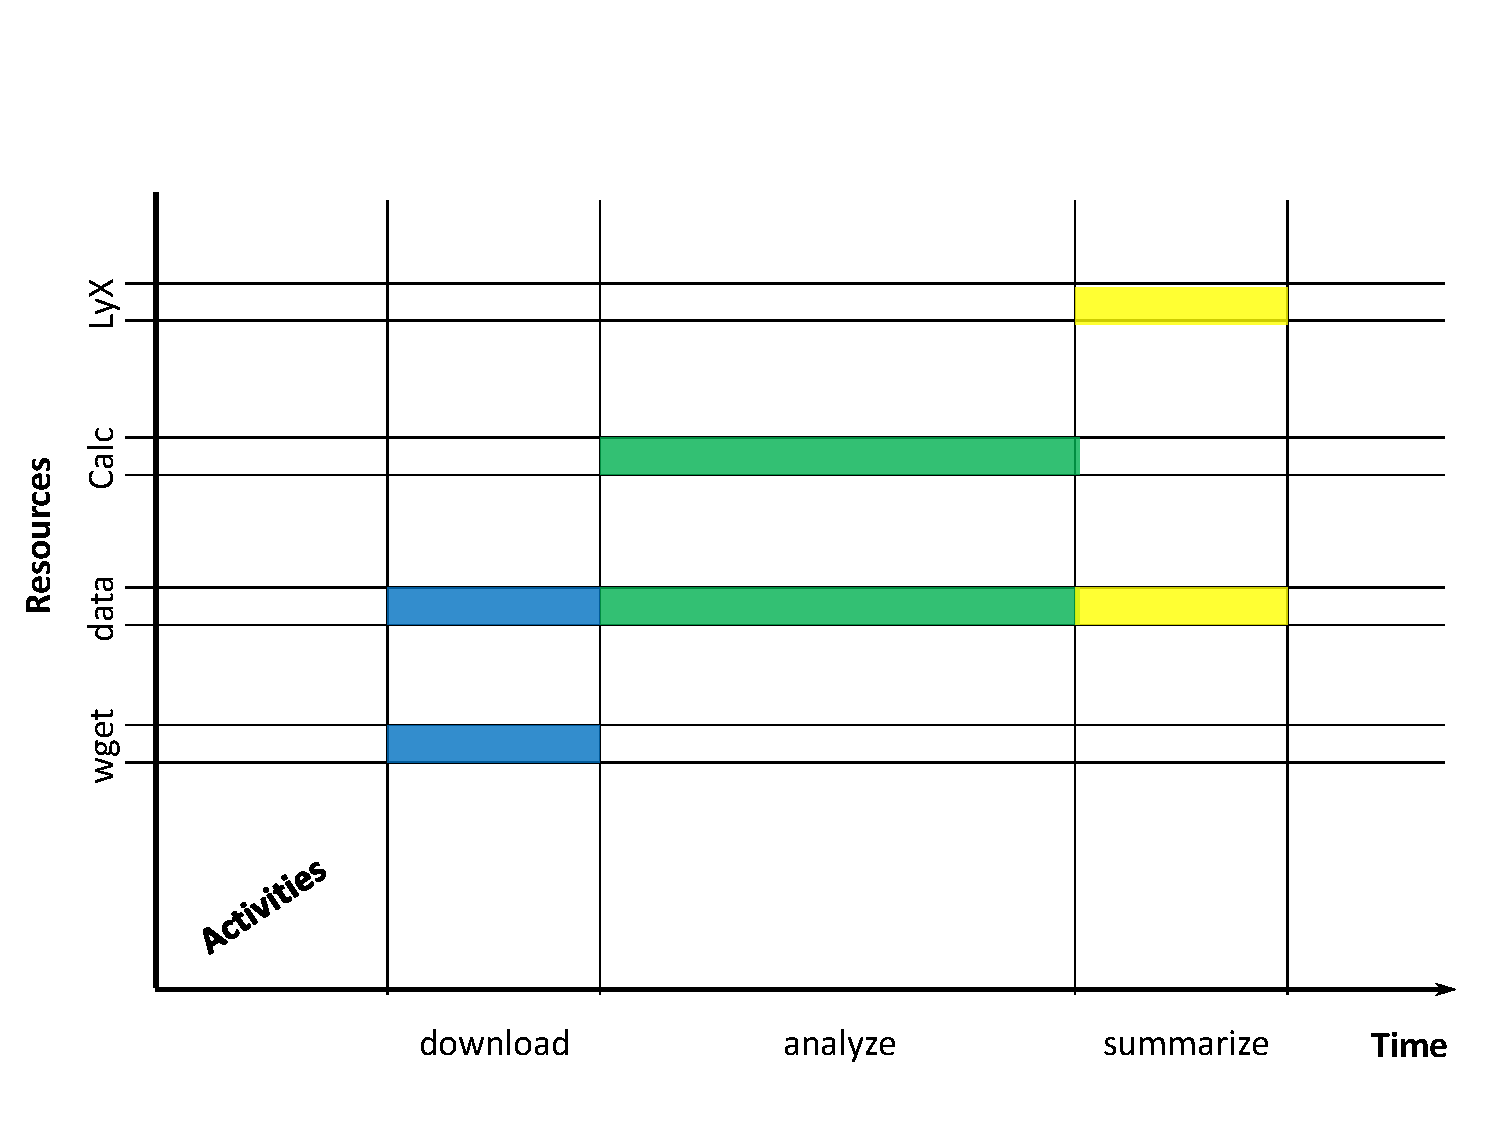
\includegraphics[scale=0.5]{prov-pieces}
\caption{How provenance information scatters throughout a table creation process}
\end{figure}
All these pieces of information can be captured by the authors if they are informed of the list of 
information items they need to record and they pay sufficient attention at certain time points where 
certain information pieces are available, but to capture them, the authors would quite often get 
distracted from their writing and table creation work. Given that doing research based on data is 
resource intensive and requires concentration, capturing provenance during writing brings no 
immediate benefit but lowers the productivity of the authors, so authors do not have incentives to 
record provenance unless they are required to do so. Even if they really would like to record all the 
details of the computational experiments they are carrying out, they are highly likely to miss some 
pieces of provenance that are not so obvious to and cannot be remembered later by human beings. 
%The benefit of having provenance information captured and properly stored comes later when some readers of the publication would like to better understand, validate and/or reproduce the published results, usually with an intention to use the result producing software for further research.

%So we see that provenance of research publication preparation shows its importance some time after 
%the publications have been created, although its importance has already been widely recognized by 
%readers and the future selves of authors. The problem is that provenance gets lost, piece by piece, 
%after the creation of publications, at a rate depending on how well the authors keep or memorize the 
%details of the publication preparation process.

\section{Possibility of developing tools to alleviate the situation}
We argue that it is possible to develop tools to alleviate the situation that important provenance gets lost due to lack of timely capturing. These tools should have the following features.
\begin{itemize}
\item \emph{Knowledge of provenance.} i.e., they have the knowledge of provenance that is necessary to capture.
\item \emph{Automatic capturing mechanism.} i.e., they support a provenance capturing mechanism that requires very little explicit input from the authors.
\item \emph{Sufficient functionality.} i.e., they support a wide range of functions authors need to perform computational experiments and to prepare research publications.
\end{itemize}
We discuss the possibility of these tools based on the features they should have.

Knowledge of provenance could be encoded and stored in these tools, e.g., in the form of an ontology. 
Existing workflow systems that enable replications of computational experiments already have the 
necessary knowledge of provenance, which our tools could inherit.

The automatic capturing mechanism is possible to implement because information about data, their steward 
activities, and agents is all available, or could be adapted to become available to certain software 
agents, since most of the operations of the computational experiments the authors perform are carried 
out with software. (Exceptions include data being noted down or copied with a pen on a piece of paper, 
but even in this case, if the authors adapt to the use of software tools and input/copy data with such 
tools on the hard drive, the automatic capturing mechanism would apply.)

To be specific, we go over the 
listed provenance items in the running example mentioned above. 
\begin{itemize}
\item Information about the original data such as its download URL is known by the download software, 
because the software needs the URL to download the data. 
\item So is the starting and ending times of the downloading activity. 
\item The user account system knows who downloads the data. 
\item The API documentation of the data analysis software package is available as part of the software 
package. 
\item Information about software parameter values and function calls is known to the software agents who 
configure the software and invoke these functions. In the case where the users need to edit a 
configuration file to change software parameter values, a software agent that can do these edits with 
function invocations could be introduced, which knows the parameter values used for each function call.
\item The person, the software and the times related to the table making activity are known by the user 
account system and the table making software itself.
\end{itemize}
%We argue that only physical, syntactical and semantic changes of data are activities worth our attention. Data representation efforts such as making the summary table have nothing to do with replicating the final results, which is a special kind of data, thus creating the representations of results does not need to be included in the provenance of the results.

Sufficient functionality is guaranteed because provenance aware versions of the existing software based on proper domain ontologies that performs data steward activities can be developed. Such software has all the functions current authors need to produce research publications. (They are just using the provenance unaware existing software to prepare research publications now.) 

To wrap up, our provenance capturing tools are provenance aware versions of existing tools used by authors of research publications. These tools get the knowledge of necessary provenance needed from the domain ontologies, and capture provenance as the authors are using the software to prepare publications -- no need to ask the authors to explicitly note down anything they have done because all they have done are already captured at the time of doing.

\section{Contributions of this thesis}
\comment{copied from abstract, review needed.}

In this thesis, we propose a paradigm of preparing research publications to overcome all the problems associated with provenance capturing in the preparing process, which is to create publications with libraries that transparently capture the proper provenance information on a portable platform.

The proper provenance information to be captured is defined in an ontology designed to model the preparing process of research publications. Although there are workflow models developed for capturing provenance in computational experiments \cite{groth2006architecture, groth2009recording}, models for provenance in publication preparation are not found. Unlike models for computational experiments, the ontology presented in this thesis pays special attention to the human factor in the process, which is a significant feature of the publication preparing process compared with the computational experiment workflows. The provenance capturing mechanism is driven by the ontology.

A portable platform is a software package or a Web application that runs on some environment that is available on all the popular computational systems, such as a Java program which runs on the Java Virtual Machine, a Python program which runs with the Python interpreter, or a Web based application written in HTML, JavaScript and/or PHP scripts which runs on any of the mainstream Web browsers. Preparing research publications based entirely on a portable platform eliminates the necessity of capturing provenance information down to the computer system level. Two desirable features for the platform are that 1) it should supply all the functions needed in creating research publications, and 2) these functions can be used in a way that is similar to the software packages the author is used to working with. To ensure the first feature, the platform needs to be extensible, better if it already has a strong development community to supply a plethora of evolving modules. The second feature requires that the platform supports popular interactive editing modes widely accepted in the research community. Examples include those seen in research software packages such as MATLAB and R.

Transparent provenance capturing means the authors using the platform are not exposed to the provenance information model that drives the capturing mechanism, which is triggered each time a publication preparing action is taken, e.g., when a block of manuscript is written, when some data are downloaded from an external source, or when a plot is created by calling a library function with the downloaded data. Capturing provenance information in this way eliminates the need to ask the authors to explicitly input provenance information. It also removes from the authors the burden of learning what provenance information to capture or communicating with people who are familiar with provenance capturing.

Contributions of this thesis are:
\begin{itemize}
\item the creation of an ontology for capturing provenance in the process of research publication preparation;
\item the proposal of a provenance capturing mechanism driven by the ontology. The mechanism makes the provenance capturing actions transparent to the authors of research publications; and 
\item the implementation of a provenance aware publication preparing platform prototype that reflects most of the desired features for the proposed provenance capturing mechanism.


%%% Local Variables: 
%%% mode: latex
%%% TeX-master: t
%%% End: 
